\documentclass[../main]{subfiles}

\begin{document}

\chapter{Schwarzian derivatives and cylinder maps}\label{cha:bonifant-milnor}

In this chapter, we follow the exposition by \textcite{bonifantSchwarzianDerivativesCylinder2008} on a family of endomorphisms of a cylinder.

\section{Cross ratios and the Schwarzian derivative}

Suppose we start with a field \(\mathbb{K}\) and, not being happy with the fact that we cannot divide by zero, decide to add a point at infinity; this gives us the \textit{projective line} \(P^1(\mathbb{K}) = \mathbb{K} \sqcup \{ \infty \}\), whose arithmetic operations are the same as those of \(\mathbb{K}\) except for the additional rules \(\frac{1}{0} = \infty\), \(\frac{1}{\infty} = 0\), \(x \cdot \infty = \infty\) if \(x \neq 0\), and \(x + \infty = \infty\) if \(x \neq \infty\).
It's not possible to define such operations everywhere without introducing inconsistent rules, so the operations are partial --- we cannot multiply \(\infty \cdot 0\) or add \(\infty + \infty\).

Our new space \(P^1(\mathbb{K})\) has an interesting property: given \(z \in P^1(\mathbb{K})\), we have three types of operations that we can apply to \(z\): translations \(z \mapsto z + x\), where \(x \in \mathbb{K}\), homotheties \(z \mapsto xz\) for \(x \in \mathbb{K} \setminus \{ 0 \}\), and the inverse \(z \mapsto 1/z\), which was not defined before if \(z = 0\), but now makes sense for every \(z\). These three families of actions, which are invertible, generate the \textit{group of homographies} with coefficients in \(\mathbb{K}\).

A second way to construct \(P^1(\mathbb{K})\), which makes the role of the group of homographies as a symmetry group of this space even clearer, is to think of the space of ``formal fractions'', that is, pairs of numbers \((x,y)\), where \(x, y \in \mathbb{K}\) are not both zero, where we identify ``equivalent fractions'', in the sense that \((\lambda x, \lambda y) \sim (x, y)\) for every \(\lambda \in \mathbb{K} \setminus \{ 0 \}\). The quotient by this equivalence relation gives us \(P^1(\mathbb{K})\) as the space of lines passing through the origin of the vector space \(\mathbb{K}^2\), and the operations are like fraction operations: \((x,y) + (z,w) = (wx + yz, yw)\), \((x,y) \cdot (z,w) = (xz, yw)\), and \((x,y)^{-1} = (y,x)\). Despite being seemingly more complicated, the interesting fact about this construction is that it emphasizes how the symmetry group of the space \(\mathbb{K}^2\), the linear group \(\GL_2(\mathbb{K})\), naturally induces a symmetry group on the quotient, the projective group \(\PGL_2(\mathbb{K})\), which is precisely the group of homographies.

This group is a quotient of \(\GL_2(\mathbb{K})\) by a subgroup of dimension \(1\), so it has dimension \(3\). Furthermore, it is \(3\)-transitive: given two sets of three distinct points in \(P^1(\mathbb{K})\), there exists an element \(g \in \PGL_2(\mathbb{K})\) that takes the first set to the second. But not only that, \(P^1(\mathbb{K})\) has three special points: \(0\), \(1\), and \(\infty\). Thus, given \(x_1,x_2, x_3 \in P^1(\mathbb{K})\) distinct, we can ask which \(g \in \PGL_2(\mathbb{K})\) such that \(g(x_1) = \infty\), \(g(x_2) = 0\), and \(g(x_3) = 1\). With some calculations, we arrive at
\begin{equation*}
  g(z) = \frac{(x_2 - z)(x_3 - x_1)}{(x_1 - z)(x_3 - x_2)}
\end{equation*}
The \emph{cross ratio} of four points \(x_{0},x_1,x_2,x_3\) is the value of \(g(x_0)\) for the element \(g\) of the homography group that sends \(x_1 \mapsto \infty\), \(x_2 \mapsto 0\), and \(x_3 \mapsto 1\).
\begin{definition}[Cross ratio]
  \begin{equation*}
    \rho(x_0,x_1,x_2,x_3) = \frac{(x_2 - x_0)(x_3 - x_1)}{(x_1 - x_0)(x_3 - x_2)}
  \end{equation*}
\end{definition}

\begin{definition}
  Let \(\f \colon I \to I'\) be a \(\Cs[d = 3]\) diffeomorphism between two intervals of the real line.
  The \emph{Schwarzian derivative} of \(\f\) is the function
  \begin{equation*}
    \SchD\f = \frac{\f[der = 3]}{\f[der = 1]} - \frac{3}{2}\rpar*{\frac{\f[der = 2]}{\f[der = 1]}}^2.
  \end{equation*}
\end{definition}
We shall write \(\SchD f \prec 0\) if there exists a dense open set \(U \subseteq I\) such that \(\SchD f(y) < 0\) for every \(y \in U\). Similarly, we write \(\SchD f \succ 0\) if there exists \(U \subseteq I\) open and dense such that \(\SchD f(y) > 0\) for every \(y \in U\).

The Schwarzian derivative has some important properties that we highlight in the Proposition below, vide \cite[Proposition B.1]{bonifantSchwarzianDerivativesCylinder2008}.

\begin{proposition}\label{prop:schwarzian}
  The Schwarzian derivative has the following properties:
  \begin{enumerate}
  \item\label{prop:schwarzian:item:1}
    The Schwarzian is a second-order derivation~\cite{ovsienkoSchwarzianDerivative}
    
    If \(\mathcal{S}f \succ 0\) and \(\mathcal{S}g \succ 0\), then \(\mathcal{S}(f \circ g) \succ 0\), and similarly for \(\prec 0\). Moreover, if \(\mathcal{S}f \equiv 0\), then \(\SchD{f \circ g} = \SchD g\), and if \(\SchD g \equiv 0\), then \(\SchD{f \circ g} = (\SchD f) \circ g\).
  \item If \(\mathcal{S}f \prec 0\), then \(\mathcal{S}f^{-1} \succ 0\). 
  \item\label{prop:schwarzian:item:3} \(\SchD f \prec 0\) if, and only if, \(\varphi(y) = 1/ \sqrt{\lvert f'(y) \rvert}\) is strictly convex.
  \item \(\SchD f \equiv 0\) if, and only if, \(f\) is a fractional linear transformation.
  \end{enumerate}
\end{proposition}

\begin{proof}\hfill
  \NewObject\IFun\fg{f \circ g}
  \begin{enumerate}
  \item We have
    \begin{equation*}
      \SchD{\fg} = \frac{\fg[spar, der = 3]}{\fg[spar, der = 1]} - \frac{3}{2}\rpar*{\frac{\fg[spar, der = 2]}{\fg[spar, der = 1]}}^2.
    \end{equation*}
    By the Faà di Bruno's formula~\cite[479]{tortoliniAnnaliDiScienze1855} in its combinatorial form,
    \begin{equation*}
      {(f\circ g)^{(n)}(x)=\sum _{\pi \in \Pi }f^{(\left|\pi \right|)}(g(x))\cdot \prod _{B\in \pi }g^{(\left|B\right|)}(x)}
    \end{equation*}
    where the sum is taken over the set \(\Pi\) of all partitions of \(\set{1,\dots,n}\), and \(B \in \pi\) means \(B\) is an element of the partition \(\pi\) (therefore, a subset of \(\set{1,\dots,n}\)).

    Specializing Faà di Bruno's formula to \(n = 1, 2, 3\), we have
    \begin{gather*}
      (f \circ g)' = (f' \circ g) \cdot g'\\
      (f \circ g)'' = (f'' \circ g) \cdot (g')^2 + (f' \circ g) \cdot g''\\
      \fg[spar, der = 3] = (\f[der = 3] \circ g) \cdot (g')^3 + 3(f'' \circ g) \cdot g'' \cdot g' + (f' \circ g) \cdot \IFun{g}[der = 3]
    \end{gather*}
    and thus 
    \begin{equation}\label{sch-comp}
      \begin{aligned}[b]
        \SchD{\fg} &=
                     \begin{multlined}[t]
                       \frac{(\f[der = 3] \circ g) \cdot (g')^3 + 3(f'' \circ g) \cdot g'' \cdot g' + (f' \circ g) \cdot \IFun{g}[der = 3]}{(f' \circ g) \cdot g'}\\ - \frac{3}{2}\rpar*{\frac{(f'' \circ g) \cdot (g')^2 + (f' \circ g) \cdot g''}{(f' \circ g) \cdot g'}}^2
                     \end{multlined} \\
                   &=
                     \frac{(\f[der = 3] \circ g) \cdot (g')^2}{f' \circ g} + 
                     3\frac{(f'' \circ g) \cdot g''}{f' \circ g} + 
                     \frac{\IFun{g}[der = 3]}{g'}
                     - \frac{3}{2}\rpar*{\frac{(f'' \circ g) \cdot g'}{f' \circ g} +
                     \frac{g''}{g'}}^2\\
                   &=\rpar*{
                     \frac{\f[der = 3] \circ g}{f' \circ g}
                     - \frac{3}{2}\rpar*{\frac{f'' \circ g}{f' \circ g}}^2}\cdot (g')^2 + 
                     \frac{\IFun{g}[der = 3]}{g'}
                     - \frac{3}{2}\rpar*{\frac{g''}{g'}}^2\\
                   &= (\SchD f) \circ g \cdot (g')^2 + \SchD g.
      \end{aligned}
    \end{equation}
    Since \(g\) is a diffeomorphism, \(g'(x) \neq 0\) for all \(x \in I\), and therefore \((g')^2 > 0\). In particular, \(g\) is a homeomorphism, so that if \(\SchD f(x) > 0\) for all \(x\) the open dense set \(U\), and \(\SchD g(x) > 0\) in the open dense set \(V\), then \(\SchD{f \circ g} > 0\) in the open dense set \(g^{-1}(U) \cap V\). Similarly, from \cref{sch-comp} we see that if \(\SchD f \equiv 0\), then the first term is zero, therefore \(\SchD{f \circ g} = \SchD g\).
  \item Applying \cref{sch-comp} to \(\Id = f^{-1} \circ f\), we see that
    \begin{equation*}
      0 = \SchD{\Id} = (\SchD f^{-1}) \circ f \cdot (f')^2 + \SchD f,
    \end{equation*}
    and by the same argument of the paragraph above, we conclude \(\SchD f \prec 0 \iff \SchD f^{-1} \succ 0\).
    \item Since \(f\) is a diffeomorphism between intervals, either \(f' > 0\) or \(f' < 0\). As a first step, assume \(f' > 0\). Taking the second derivative of \(\varphi(y) = 1/ \sqrt{f'(y)} = f'(y)^{-1/2}\),
    \begin{equation*}
      \varphi'' = \rpar*{-\frac{1}{2}\rpar{f'}^{-3/2}\cdot{\f''}}' =
      \frac{3}{4}(f')^{-5/2}\cdot (f'')^2 - \frac{1}{2}(f')^{-3/2}\cdot \f[der = 3].
    \end{equation*}
    Thus
    \begin{equation}
      2{\varphi''}/{\varphi} = 
      \frac{3}{2}(f')^{-4/2}\cdot (f'')^2 - (f')^{-2/2}\cdot \f[der = 3] =\frac{3}{2}\rpar*{\frac{\f[der = 2]}{\f[der = 1]}}^2 - \frac{\f[der = 3]}{\f[der = 1]}  = - \SchD f.\label{sch-rel}
    \end{equation}
    From this, and noticing that \(\varphi > 0\), we see that if \(\SchD f(x) < 0\) if and only if \(\varphi''(x) > 0\). A \(C^2\) function \(\varphi : I \to \RR\) will be strictly convex if and only if  \(\varphi'' \ge 0\) and \(\varphi''\) does not vanish on any open interval,
    so \(\SchD f \prec 0\) implies that \(\phi''\) is positive in an open dense set, thus strictly convex. Reciprocally, if \(\varphi\) is strictly convex, then the set \(\set{x \where \varphi''(x) > 0} = \set{x \where \SchD f(x) < 0}\) is open and its complement does not contain any open interval, and therefore is dense.

    If \(f' < 0\), we define \(g \colon I \to - I'\), \(g(y) = - f(y)\), so that \(g' > 0\) and we fall back to the previous case. The argument is finished by noticing that \(\SchD g =  \SchD f\) and \(1/ \sqrt{\abs{f'}} = 1/\sqrt{\abs{g'}}\).
  \item From \cref{sch-rel}, we see that \(\SchD f \equiv 0 \iff \varphi'' \equiv 0\). This, in turn, is equivalent to \(\varphi\) being linear, say \(\varphi(y) = cy + d\). We thus have
    \begin{equation*}
      f'(y) = \frac{1}{(cy + d)^2}.
    \end{equation*}
    Integrating both sides, by the Fundamental Theorem of Calculus we have
    \begin{equation*}
      f(y) - f(a) = \int_a^y \frac{1}{(ct + d)^2} \;dt = \frac{1}{c}\rpar*{\frac{1}{ca + d} - \frac{1}{cy + d}} = \frac{y - a}{c(ca + d)y + d(ca + d)}
    \end{equation*}
    which is a fractional linear transformation, as desired.
  \end{enumerate}
\end{proof}

\begin{lemma}\label{lem:sch-fixed-pts}
  If \(f \colon I \to I'\) is \(C^3\) and \(\SchD f \prec 0\), then \(f\) has at most three fixed points. When it has three fixed points, the middle one is strictly repelling and the other two are strictly attracting.
\end{lemma}

\begin{proof}
  Suppose \(f\) had four fixed points \(y_1 < y_2 < y_3 < y_4\). By the Mean Value Theorem, in each of the three open intervals \((y_i,y_{i + 1})\), for \(i = 1,2,3\), we would have a point  \(c_i \in (y_i,y_{i + 1})\) where \(f'(c_i) = 1\). But this is impossible, since by \cref{prop:schwarzian:item:3} \(\varphi(y) = 1/ \sqrt{\lvert f'(y) \rvert}\) is strictly convex, which would imply \(\varphi(c_2) < \varphi(c_1) = \varphi(c_3) = 1\).

  Now, suppose there are exactly three fixed points \(y_1 < y_2 < y_3\). By the same reasoning, there are two points \(c_1 \in (y_1,y_2)\) and \(c_2 \in (y_2, y_3)\) where \(\varphi(c_1) = \varphi(c_2) = 1\). Knowing that \(\varphi\) is strictly convex, this implies \(\varphi(y_2) > 1\) and \(\varphi(y_1), \varphi(y_3) < 1\), and therefore \(\abs{f'(y_2)} < 1\) and \(\abs{f'(y_1)},\abs{f'(y_3)} > 1\).
\end{proof}

\begin{lemma}\label{lem:sch-cross-increase}
  If \(f \colon I \to I'\) is \(C^3\), then \(\SchD f \prec 0\) if, and only if, \(f\) increases cross ratios, in the sense that \(\rho(f(y_{1}),f(y_2),f(y_3),f(y_4)) > \rho(y_{1},y_2,y_3,y_4)\) for all \(y_1 < y_2 < y_3 < y_{4}\).
\end{lemma}

\begin{proof}
  Given \(y_1 < y_2 < y_3 < y_{4}\), let \(\varphi\) be the linear fractional transformation that sends \(f(y_1)\) to \(y_1\), \(f(y_2)\) to \(y_2\) and \(f(y_4)\) to \(y_4\). Since from \cref{prop:schwarzian}, we have that \(\SchD{\varphi \circ f} = \SchD f\), and we know fractional linear transformations also preserve cross-ratios, without loss of generality we may assume that \(f\) itself fixes \(y_1,y_2\) and \(y_4\). Now, by \cref{lem:sch-fixed-pts}, \(f(y) > y\) on the interval \(\interval[open]{y_2}{y_4}\), and therefore \(f(y_3) > y_3\). It thus follows easily by the definition of cross-ratios that \(\rho(f(y_{1}),f(y_2),f(y_3),f(y_4)) > \rho(y_{1},y_2,y_3,y_4)\).
\end{proof}

\begin{lemma}\label{lem:bound-deriv-schwarz}
  If \(f \colon I \to I\) is a diffeomorphism that preserves orientation and \(\SchD f \prec 0\), where \(I = [a,b]\), then \(f'(a)f'(b) < 1\).
\end{lemma}

\begin{proof}
  Let's consider the case where \(f'(a) = f'(b)\) first. If we had \(f'(a)^2 = f'(b)^2 = f'(a)f'(b) \ge 1\), then \(\varphi(a) = \varphi(b) \le 1\) which by strict convexity of \(\varphi\) implies \(\varphi|_{(a,b)} < 1\). This, in turn, means that \(f'|_{(a,b)} < 1\), which (by the mean value theorem) is not possible for a diffeomorphism that sends an interval to itself.

  The general case is shown by noticing that if we define the function \(g = r \circ f \circ r \colon I \to I\), where \(r(x) = a + b - x\) (and thus \(g\) is the reflection of \(f\) along the anti-diagonal), then \(g'(a) = f'(b)\) and \(g'(b) = f'(a)\). By the chain rule,
  \begin{equation*}
    (f \circ g)'(a) = (f \circ g)'(b) = f'(a)f'(b),
  \end{equation*}
  and by \cref{prop:schwarzian:item:1}, \(\SchD{f \circ g} \prec 0\) because \(\SchD{r} \equiv 0\) and thus \(\SchD{g} = \SchD{f} \circ r \prec 0\).
\end{proof}

Note that by \cref{prop:schwarzian}, analogous results to the last two lemmas hold if \(\SchD f \succ 0\). For example, if \(\SchD f \succ 0\) then \(f\) decreases cross ratios and \(f'(0)f'(1) > 1\).

%%% REVISED

\section{Skew products}

We call a map \(F \colon X \times Y \to X \times Y\) a \emph{skew product} if it is of the form \(F(x,y) = (g(x), f_x(y))\) for some \(g \colon X \to X\) and a family of functions \(\{ f_x \}_{x \in X}\), \(f_x \colon Y \to Y\). We are interested in the case where \(X\) is a compact metric space with the Borel \(\sigma\)-algebra, \(g \colon X \to X\) is a continuous map preserving an ergodic probability measure \(\mu \in \Meas{X}\), \(Y = I\) is the interval \([0,1]\), and \(f_x \colon I \to I\) are \(C^3\) diffeomorphisms preserving orientation. We will see how, depending on the Schwarzian derivative of the maps \(f_x\), we observe different behaviors of the dynamics with respect to the invariant measures \(\nu_0 = \mu \otimes \delta_0\) and \(\nu_1 = \mu \otimes \delta_1\). Note that for \(i \in \{ 0,1 \}\), \(\supp \nu_i = \mathcal{A}_i\), where \(\mathcal{A}_i = X \times \{ i \}\) are the upper and lower ``boundaries'' of \(X \times I\).
Let \(\mathcal{B}_i = \mathcal{B}(\nu_i)\) be the basins of the respective measures.

To simplify notation, let's denote by \(f_x^{n}(y)\) the second coordinate of \(F^n(x,y)\), that is, \(f_x^{n} = f_{g^{n - 1}(x)} \circ \cdots \circ f_x\).

\begin{lemma}\label{lem:basin-segment}
  If \((x, y_1) \in \mathcal{B}_0\), then \((x,y_2) \in \mathcal{B}_0\) for all \(y_2 \leq y_1\). Similarly, if \((x, y_1) \in \mathcal{B}_1\), then \((x,y_2) \in \mathcal{B}_0\) for all \(y_2 \geq y_1\).
\end{lemma}

\begin{proof}
  We will prove the case \(i = 0\), as the situation is symmetric. Let \((x,y_1) \in \mathcal{B}_0\) and \(y_2 \leq y_1\). If \(\varphi \in \Cs{X \times I}\), and \(\varepsilon > 0\), by the uniform continuity of \(\varphi\), there exists \(\delta > 0\) such that \(y < \delta\) implies \(\lvert \varphi(x,0) - \varphi(x,y) \rvert < \varepsilon\) for all \(x \in X\). Since \(U = X \times \interval[open right]{0}{\delta}\) is a continuity set for \(\nu_0\) and \(e_n(x,y_2) \to \nu_0\), by \nameref{thm:portmanteau}
    \newcommand{\timeinU}{\frac{1}{n}\# \set{ 0 \leq i < n \where f_x^n(y_2) < \delta }}
    \[\lim_{n \to \infty} e_n(x,y_2)(U) = \nu_0(U) = 1.\]
    Define \(\tau_n = e_n(x,y_2)(U) = \timeinU\).
    Note that if \(f_x^n(y_2) < \delta\), then \(f_x^n(y_1) < \delta\) since the diffeomorphisms preserve orientation. Thus,
    \begin{align*}
      \lvert e_n(x,y_1)(\varphi) - e_n(x,y_2)(\varphi) \rvert
      &\leq \frac{1}{n}\sum_{i = 0}^{n - 1}\abs[\big]{\varphi(g^n(x),f_x^{n}(y_1)) - \varphi(g^n(x),f_x^{n}(y_2))}\\
      &\leq \varepsilon \tau_n + 2 \lVert \varphi \rVert_{\infty} (1 - \tau_n).
    \end{align*}
    Since \(\tau_n \to 1\), there exists \(N\) such that \(n \geq N\) implies that the right side is less than \(2 \varepsilon\), hence both integrals on the left converge to \(\nu_0(\varphi)\).
\end{proof}

\section{Transversal Lyapunov exponents}

To each point \((x,y)\) of either boundary \(\mathcal{A}_i\), for \(i \in \set{0,1}\), we can associate a number that expresses the average expansion rate of tangent vectors along the direction normal to the skew product boundary. This is a specific case of the general definition of Lyapunov exponents, whose existence is given by the Oseledets theorem.

\begin{definition}[Transversal Lyapunov exponent]
  \begin{equation*}
    \Lyap_{\mathcal{A}_i}(x) = \lim_{n \to \infty}\frac{1}{n} \log \abs*{ \partial_y F^{n}(x,i) }.
  \end{equation*}
\end{definition}
By the product rule, and noting that \(\set{0,1}\) are fixed points of the fiber diffeomorphisms, the right side of the equation above can be rewritten as
\begin{equation*}
  \lim_{n \to \infty}\frac{1}{n} \sum_{k = 0}^{n - 1} \log \abs*{\partial_y F(g^k(x),i)}
  = \lim_{n \to \infty}\frac{1}{n} \sum_{k = 0}^{n - 1} \log f_{g^k(x)}'(i).
\end{equation*}
Thus, by the ergodicity of \(\mu\)  for \(g\) and the Birkhoff ergodic theorem,  for \(\mu\)-almost every \(x \in X\) it holds that
\begin{equation}\label{eq:trav-lyap}
  \Lyap_{\mathcal{A}_i}(x) = \int \log f_{x}'(i) \;d \mu(x),
\end{equation}
and we shall denote this common value by \(\Lyap(\mathcal{A}_i)\).

The version of the statement below is slightly more general than the corresponding one in~\cite[lema A.1]{bonifantSchwarzianDerivativesCylinder2008}, that asks for \(F\) to be \(C^2\). In our context, \(F(x,y) = (g(x),f_x(y))\) where \(g\) is an ergodic map for \(\mu\) and \(f_x \in C^1[0,1]\) for all \(x\). In particular, if \((x,y) \mapsto f'_x(y)\) is continuous, the following equicontinuity hypothesis is satisfied. 
\begin{lemma}\label{lem:lyap-basin-posmeas}
  If the family \(\{ f_x' \}_{x \in X}\) is equicontinuous at \(i \in \{ 0,1 \}\) and \(\Lyap(\mathcal{A}_i) < 0\), then the basin of \(\mu \otimes \delta_i\) has positive \(\mu \otimes \Leb\) measure.  Conversely, if \(\Lyap(\mathcal{A}_i) > 0\), then the corresponding basin has null measure.
\end{lemma}

\begin{proof}
  We will assume \(i = 0\). Let \(\varepsilon > 0\) be such that
  \begin{equation*}
    \int \log(f_x'(0) + \varepsilon) \;d\mu(x) < 0.
  \end{equation*}
  Let \(a(x) = \log(f_x'(0) + \varepsilon)\). By the Birkhoff ergodic theorem, for \(\mu\)-almost every \(x \in X\)
  \begin{equation*}
    \lim_{n \to \infty}\frac{1}{n}\sum_{k = 0}^{n - 1} a(g^k(x)) = 
    \int a(x) \;d\mu(x) < 0,
  \end{equation*}
  which implies \(\lim_{n \to \infty}\sum_{k = 0}^{n - 1} a(g^k(x)) = -\infty\). This means that the function
  \begin{equation*}
    A(x) = \max_{n \geq 1}\sum_{k = 0}^{n - 1} a(g^k(x)) \geq 0
  \end{equation*}
  is well-defined in almost every \(x\).
  
  By equicontinuity, there is \(\delta>0\) such that \(0 \le y \le \delta\) implies \(f_x'(x) \le f'_x(0) + \varepsilon\) for all \(x \in X\). Thus, if \(y < \delta e^{-A(x)}\), we claim that
  \begin{equation}\label{eq:max-ind}
    f_x^n(y) \leq \exp\rpar*{\sum_{k = 0}^{n - 1}a(g^k(x)) - A(x)}\delta \leq \delta.
  \end{equation}
  is true by induction. Indeed, the \(n = 0\) case follows from the hypothesis on \(y\), and if~\eqref{eq:max-ind} is true for \(n\), then by the mean value theorem,
  \begin{align*}
    f_x^{n + 1}(y) &\leq \rpar[\Big]{\max f'_{g^{n}(x)}([0, f^n_x(y)])} f_x^n(y) \\
                   &\leq (f'_{g^{n}(x)}(0) + \varepsilon)f_x^n(y)\\
                   &\leq \exp\rpar*{a(g^{n}(x)) + \sum_{k = 0}^{n - 1}a(g^k(x)) - A(x)}\delta.
  \end{align*}
  Since \(\lim_{n \to \infty} \sum_{k = 0}^{n - 1}a(g^k(x)) = -\infty\), we have \(f_x^{n + 1}(y) \to 0\). Thus, if \(x \in \mathcal{B}(\mu)\) (which has full measure), then \(e_{n}(x,y) \weakto \nu_0\) whenever \(y \leq \delta e^{-A(x)}\).

  % TODO: write the converse
\end{proof}

\begin{corollary}\label{cor:schwarz-basin-pos-meas}
  If \((x,y) \mapsto \SchD f_x(y)\) is continuous and \(\SchD f_x \prec 0\) for \(\mu\)-almost every \(x \in X\), then \(\Lyap(\mathcal{A}_0) + \Lyap(\mathcal{A}_1) < 0\).
  In particular, at least one of the basins has positive measure.
\end{corollary}

\begin{proof}
  If suffices to integrate the logarithm of the inequality \(f_x'(0)f_x'(1) < 1\) from \cref{lem:bound-deriv-schwarz}, and then apply \cref{lem:lyap-basin-posmeas}.
\end{proof}

\section{Intermingled basins}

The basins of the examples we saw before are continuity sets for the volume measure --- that is, they are open sets modulo a zero volume set --- and the union of all basins have full Lebesgue measure. But should basins of attractors  constitute well-behaved sets in general? In some cases, such as for uniformly hyperbolic diffeomorphisms, this indeed the case, and there is a finite number of physical measures whose basins are continuity sets, and their union has full volume \cite{uresNonrobustnessIntermingledBasins2018}. Outside the realm uniform hyperbolicity, though,  this may not be the case --- \textcite{kanOpenSetsDiffeomorphisms1994} gave the first example of a partially hyperbolic endomorphism on a surface with two physical measures whose basins are intermingled, in the sense that for every open set \(U\), the intersection of this set with either basin has positive volume \cite{uresNonrobustnessIntermingledBasins2018}. Clearly, this implies both basins are dense in the surface, and therefore not continuity sets.

\todo{Refer to discussion in~\cite{bonattiDynamicsUniformHyperbolicity2005}}

In this section we shall describe the construction of that flavor of example in a more general setting of skew products that also encompasses the original example. As before, let \(X\) be a compact metric space, \(g \colon X \to X\) be ergodic for \(\mu \in \Meas[1]{X}\) and \(F \colon X \times I \to X \times I\) a continous skew-product endomorphism of the form \(F(x,y) = (g(x), f_x(y))\). We shall understand by  ``volume'' the reference measure \(m = \mu \otimes \Leb\). As mentioned in \cref{lem:lyap-basin-posmeas}, under some mild hypothesis for \(F\), if the transverse Lyapunov exponents at the invariant boundaries \(\mathcal{A}_i = X \times \set{i}\), given by
\begin{equation*}
  \Lyap(\mathcal{A}_i) = \int \log f_{x}'(i) \;d \mu(x)
\end{equation*}
for \(i = 0,1\) are both negative, then both basins have positive volume. Assuming this, the main property that will produce the intermingled phenomenon is the following hypothesis.
\begin{hypothesis}\label{hip:elevators}
  There exists two periodic points \(x^+\) and \(x^-\) in \(X\), of periods \(n^+, n^-\), such that for every  \(y \in (0,1)\), \(f_{x^+}^{n^+}(y) > y\) and \(f_{x^-}^{n^-}(y) < y\).
\end{hypothesis}

Note that if we define the measures \(\mu_i(A) = \Leb(A \cap \mathcal{B}_i)\), then the basins are intermingled if, and only if, \(\supp \mu_i = X \times I\) for both \(i = 0,1\). We will show this is the case for \(\supp \mu_0\), as the proof for \(i = 1\) follows by symmetry. First, we shall collect some lemmas. 

\begin{lemma}
  Given \(x \in X\), \(\supp \mu_0 \cap \{ x \} \times I\) is a segment \(\{ x \} \times [0,a_x]\).
\end{lemma}
\begin{proof}
  By \cref{lem:basin-segment}, \(\mathcal{B}_0\) is of the above form. Since we know that the support of a measure is closed, we can take \(y < 1\) such that \((x,y) \in \supp \mu_0\) and show that if \(z < y\) then \((x,z) \in \supp \mu_0\).
  Let \(U = B_{\varepsilon}(x,z)\) be a ball centered at \((x, z)\) of radius smaller than \(1 - y\), and \(V = B_{\varepsilon}(x,y)\). Note that
  \[V \cap \mathcal{B}_0 \subseteq \set{(u,v + y - z) \where (u,v) \in U \cap \mathcal{B}_0},\] so since \((x,y) \in \supp \mu_0\), and \(\Leb\) is invariant by vertical translations, \(\Leb(U \cap \mathcal{B}_0) \geq \Leb(V \cap \mathcal{B}_0) > 0\).
\end{proof}

\begin{lemma}
  The support \(\supp \mu_0\) is an invariant set, that is, \(F^{-1}(\supp \mu_0) = \supp \mu_0\).
\end{lemma}
\begin{proof}
  If \(p \in F^{-1}(\supp \mu_0)\) and \(U\) is a neighborhood of \(p\), then since \(F\) is an open map, \(F(U)\) is a neighborhood of \(F(p) \in \supp \mu_0\), so \(\mu_0(F(U)) > 0\). Since \(F\) is Lipschitz, if \(\mu_0(U)\) were \(0\), then \(\mu_0(F(U)) = \Leb(F(U) \cap \mathcal{B}_0) = \Leb(F(U \cap \mathcal{B}_0)) = 0\), which is not the case, so \(\mu_0(U) > 0\).
\end{proof}


\begin{corollary}
  \(\supp \mu_0 = X \times I\).
\end{corollary}

\begin{proof}
  Since \(\supp \mu_0\) is closed and by hypothesis, \(F^n(x^-,y) \to (x^-,0)\) for all \(y \in (0,1)\), then \(\set{0} \times I \subseteq \supp \mu_0\).
\end{proof}

\begin{proof}
  By symmetry, it is enough to show  \(\mathcal{A}_1 \subseteq K\). Let \((x,y) \in K\) be the point in the statement. 

  Inductively, we can construct a backward orbit \(\cdots \mapsto x_{-2} \mapsto x_{-1} \mapsto x_0\) of \(g\) such that \(x_{ - n - 1} \in g^{-1}(\{ x_{-n} \})\) is the closest preimage of \(x_-\). Since \(x_-\) is a repelling fixed point, the construction implies that \(x_{-n} \to x_-\), so by \cref{hip:elevators}, for every \(y \in (0,1)\) there exists \(n_0\) such that \(n \geq n_0\) implies \(f_{x_{-n}}^{-1}(y_0) > y\). In particular,
  \[y_{ - n} = f_{x_{-n}}^{-1} \circ \cdots \circ f_{x_{-1}}^{-1}(y_0)\]
  is such that \(y_{ - n} \to 1\). Since \(\supp \mu_0\) is closed and \((x_{ - n},y_{ - n}) \in F^{-n}(\supp \mu_0)\), we conclude that \((x_-, 1) \in \supp \mu_0\). Now, notice that \(E = \bigcup_{n = 0}^{\infty}g ^{-1}(\{ x_- \})\) is dense in \(X\) and \(1\) is a fixed point of the \(f_x\). Thus, \(E \times \{ 1 \} \subseteq \supp \mu_0\) and consequently \(\mathcal{A}_1 \subseteq \supp \mu_0\).
\end{proof}

\begin{corollary}\label{cor:intermingled}
  Suppose \cref{hip:elevators} holds and both basins have positive measure. Then the basins \(\mathcal{B}_0\) and \(\mathcal{B}_1\) are intermingled for the Lebesgue measure on the cylinder.
\end{corollary}

\begin{proof}
  By definition, the basins are strictly invariant sets. If we define the measures \(\mu_i(A) = \Leb(A \cap \mathcal{B}_i)\), then the basins are intermingled if, and only if, \(\supp \mu_i = X \times I\) for both \(i = 0,1\). We will show this is the case for \(\supp \mu_0\), as the proof for \(i = 1\) is analogous.

  \begin{claim}
    The support \(\supp \mu_0\) is backwards-invariant.
  \end{claim}
  Indeed, if \(p \in F^{-1}(\supp \mu_0)\) and \(U\) is a neighborhood of \(p\), then since \(F\) is an open map, \(F(U)\) is a neighborhood of \(F(p) \in \supp \mu_0\), so \(\mu_0(F(U)) > 0\). Since \(F\) is Lipschitz, if \(\mu_0(U)\) were \(0\), then \(\mu_0(F(U)) = \Leb(F(U) \cap \mathcal{B}_0) = \Leb(F(U \cap \mathcal{B}_0)) = 0\), which is not the case, so \(\mu_0(U) > 0\).

  \begin{claim}
    There exists a point \((x_0,y_0) \in \supp \mu_0 \setminus X \times \{ 0 \}\).
  \end{claim}
  Indeed, \(\mu_0(\supp \mu_0) \geq \Leb(\mathcal{B}_0) > 0\), so \(\mu_0(\supp \mu_0 \setminus X \times \{ 0 \}) > 0\) and the set cannot be empty.

  \begin{claim}
    Given \(x \in X\), \(\supp \mu_0 \cap \{ x \} \times I\) is a segment \(\{ x \} \times [0,a_x]\).
  \end{claim}
  By \cref{lem:basin-segment}, \(\mathcal{B}_0\) is of the above form. To show that the support also has this property, we can take \(y < 1\) such that \((x,y) \in \supp \mu_0\) and show that if \(z < y\) then \((x,z) \in \supp \mu_0\).
  Let \(U = B_{\varepsilon}(x,z)\) be a ball centered at \((x, z)\) of radius smaller than \(1 - y\), and \(V = B_{\varepsilon}(x,y)\). Note that \(V \cap \mathcal{B}_0 \subseteq (U \cap \mathcal{B}_0) + (0, y - z)\), and since \((x,y) \in \supp \mu_0\), \(\Leb(U \cap \mathcal{B}_0) \geq \Leb(V \cap \mathcal{B}_0) > 0\). This shows the claim.

  Now, by the first two claims and \cref{thm:inv-closed-contains-boundary}, \(\supp \mu_0\) contains both boundaries. By the last claim, it is composed of vertical segments, so it must be equal to \(X \times I\).
\end{proof}

\begin{figure}[h]
  \centering
  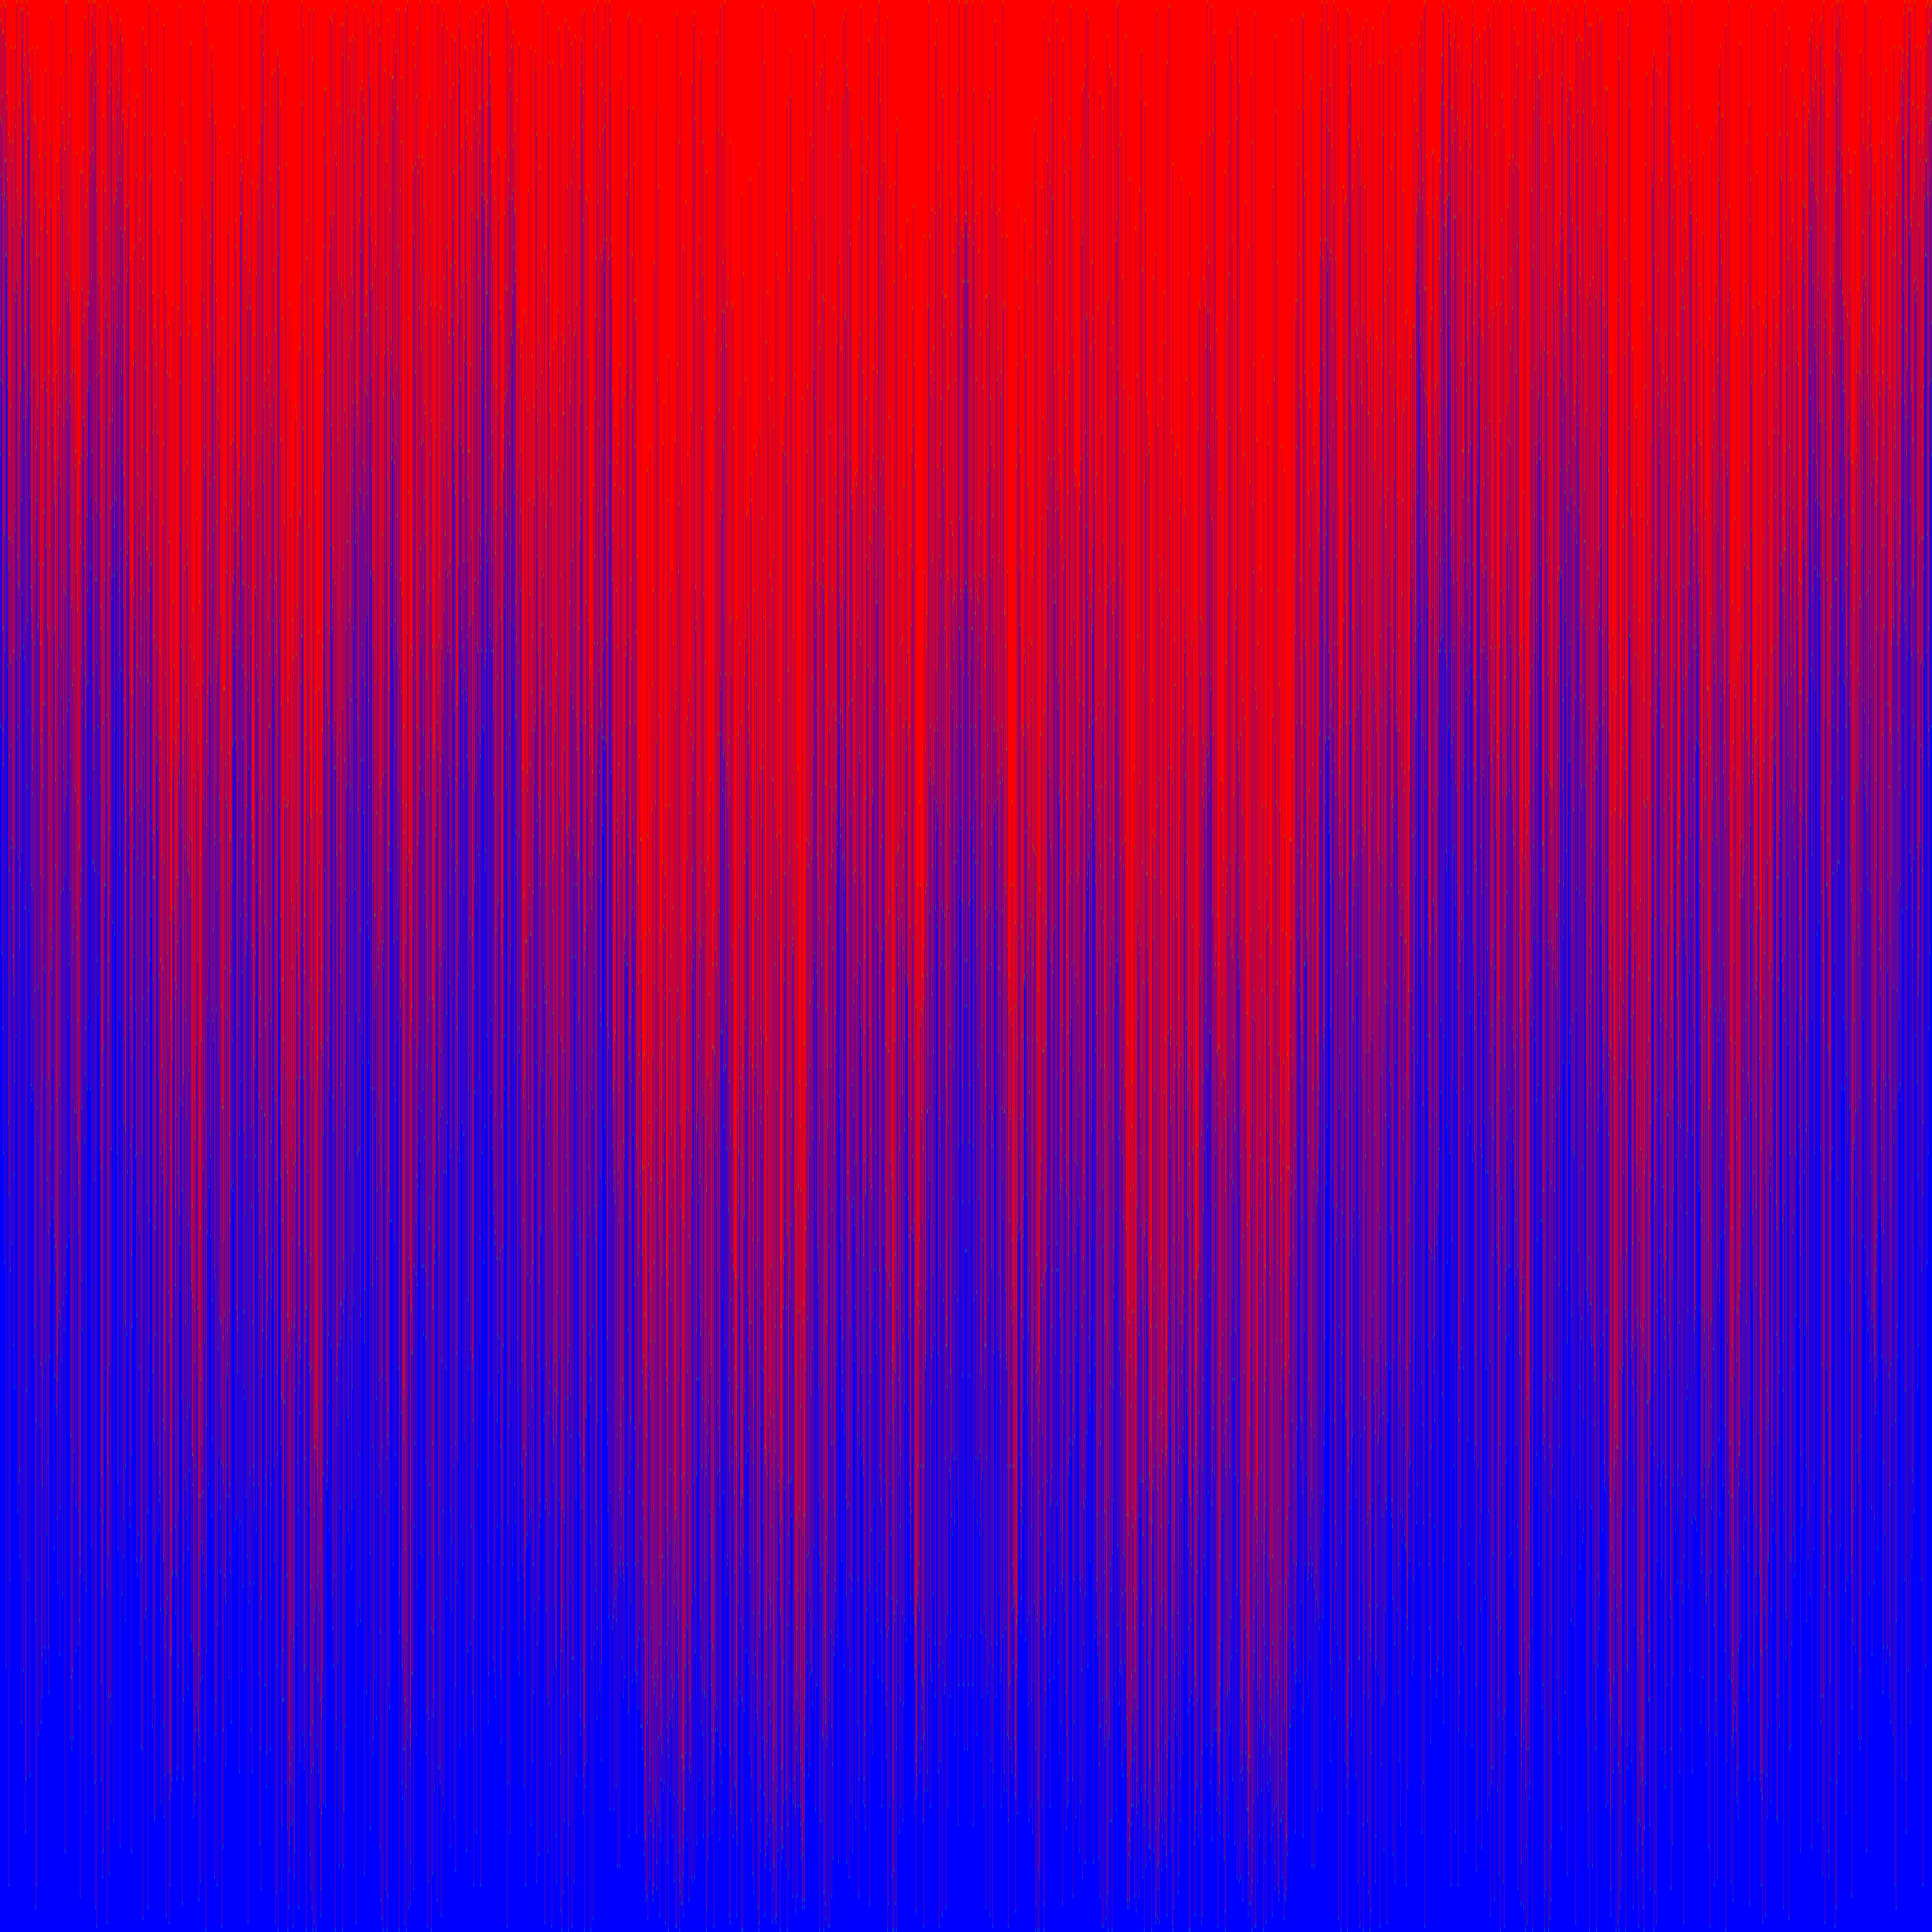
\includegraphics[width=0.35\textwidth]{../figures/intermingled}
  \caption{Picture of the basins of \cref{ex:intermingled}. It should not be taken too seriously, as it is evidently not possible to draw intermingled sets.}
\end{figure}

\begin{example}\label{ex:intermingled}
  Define \(q_a(y) = y + ay(1 - y)\) and \(p(x) = \varepsilon \cos(2 \pi x)\) for some \(0 < \varepsilon < 1\). If \(|a| < 1\), then \(q_a\) is a diffeomorphism of the interval \(I\). If \(F(x) = (3x, q_{p(x)}(y))\), then \(x^+ = 0\) and \(x^- = 1/2\) are fixed points of the map \(g(x) = 3x\) (where we identify \(S^1\) with \([0,1]\)) that satisfy \cref{hip:elevators}, because \(q_a(y) > y\) if \(a > 0\) and \(q_a(y) < y\) if \(a < 0\) for all \(y \in (0,1)\). Moreover, since \(q_a\) is a degree two polynomial, it has negative Schwarzian whenever \(a \neq 0\), and from the symmetry of \(p\) we see both basins of \(F(x,y) = (kx, q_{p(x)}(y))\) must have positive measure, because at least one of them has. So \(F\) displays intermingled basins. 
\end{example}

\section{Negative Schwarzian}

The statement of the theorem below corresponds to~\cite[Theorem 3.2]{bonifantSchwarzianDerivativesCylinder2008} without the hypothesis that both basins have positive measure. The question of whether this hypothesis could be removed was left open in the article, and the following proof shows that it is indeed unnecessary.

\begin{theorem}\label{thm:neg-schwarz-sep-graph}
  If \((x,y) \mapsto \SchD f_x(y)\) is continuous and \(\SchD f_x \prec 0\) almost everywhere in \(x \in X\), then there exists a measurable function \(\sigma \colon X \to I\) defined almost everywhere such that
  \begin{equation*}
    (x,y) \in \mathcal{B}_0 \text{ whenever } y < \sigma(x) \quad \text{and} \quad (x,y) \in \mathcal{B}_1 \text{ whenever }y > \sigma(x).
  \end{equation*}
  Consequently, the union \(\mathcal{B}_0 \cup \mathcal{B}_1\) has total \(\mu \otimes \Leb\) measure.
\end{theorem}

\begin{proof}
  We start by defining functions \(\xi_0, \xi_1 \colon X \to I\) that separate the basins in the following sense:
  \begin{equation*}
    \xi_0(x) = \sup \{ y \in I : y \in \mathcal{B}_0 \}, \qquad \xi_1(x) = \inf \{ y \in I : y \in \mathcal{B}_1 \}.
  \end{equation*}
  By \cref{lem:basin-segment}, if \(y < \xi_0(x)\) or \(y > \xi_1(x)\), the empirical measures \(e_n(x,y)\) converge to \(\nu_0 = \mu \otimes \delta_0\) or to \(\nu_1 = \mu \otimes \delta_1\), and if \(\xi_0(x) < y < \xi_1(x)\), they do not converge to either \(\nu_0\) or \(\nu_1\).
  
  It is sufficient to show that \(A = \{ x \in X : \xi_0(x) \neq \xi_1(x) \}\) has measure zero, since in this case we can define \(\sigma\) as the common value of the two functions. Suppose by contradiction that this set does not have measure zero. Since the \(f_x\) are bijective, \(A\) is an invariant set under \(g\), so the ergodicity of \(\mu\) implies that \(A\) has full measure.

  Since we are under the hypotheses of \cref{cor:schwarz-basin-pos-meas}, we can assume without loss of generality that \(\Leb(\mathcal{A}_1) > 0\). By ergodicity, we also have \(\xi_1(x) < 1\) for \(\mu\)-almost every \(x \in X\). Thus, given \(k \in \NN\), there exists \(\delta_k < 1\) such that \(E_k = \{ x \in X : \xi_1(x) < \delta_k \}\) has measure \(\mu(E_k) > 1 - 1/k\). Applying the Birkhoff ergodic theorem to the functions \(1_{E_k}\), we obtain \(B \subseteq X\) of full measure such that for all \(x \in B\) and \(k\),
  \begin{equation}\label{eq:time-small}
    \lim_{n \to \infty} \frac{1}{n} \# \set{ 0 \leq i < n \where \xi_1(g^i(x)) < \delta_k} = \mu(E_{k}) > 1 - 1/k.
  \end{equation}
  
  By the ergodicity of \(\mu\), there exists another set \(C \subseteq X\) of full measure whose empirical measures converge to \(\mu\), and since \(\SchD f_x \prec 0\) almost everywhere in \(x \in X\), there exists a set \(D\) of full measure such that \(\SchD f_{g^n(x)} \prec 0\) for all \(n \geq 0, x \in D\). Let \(x_0 \in A \cap B \cap C \cap D\) and \(y_0 \in (\xi_0(x), \xi_1(x))\), and let \(\nu \in \Meas{x,y} \setminus \{ \nu_0 \}\) be a limit point of the empirical measures different from \(\nu_0\). Note that since \(x_0 \in B\), necessarily \((\pi_X)_* \nu = \mu\), but since \(\nu \neq \nu_0\), it follows that \(\nu(X \times \{ 0 \}) < 1\). Thus, \(\supp \nu\) is not contained in \(X \times \{ 0 \}\), and there exists \(\varepsilon > 0\) such that \(U = X \times \interval[open left]{\varepsilon}{1}\) satisfies \(\nu(U) > 0\). Let \(k\) be such that \(\nu(U) > 1/k\), and \(n_j \to \infty\) such that \(\liminf_{j \to \infty} e_{n_j}(x_0,y_0)(U) > 1/k\).
  In other words, we have
  \begin{equation}\label{eq:time-big}
    \liminf_{j \to \infty} \frac{1}{n_j} \# \set{ 0 \leq i < n_j \where f_{x_0}^i(y_0) > \varepsilon} > 1/k.
  \end{equation}

  Now, consider the sequence \(r_n = \rho(0, f_{x_0}^n(y_0), f_{x_0}^n(\xi_1(x_0)), 1)\), which is well-defined and positive since \(0 < f_{x_0}^n(y_0) < f_{x_0}^n(\xi_1(x_0)) < 1\) by the definition of the points. Note also that the graph of \(\xi_1\) is strictly invariant under \(F\), so \(f_{x_0}^n(\xi_1(x_0)) = \xi_1(g^n(x_0))\).

  Since \(x \in D\), it follows by \cref{lem:sch-cross-increase} that \(r_n\) is an increasing sequence. On one hand, it is not possible for \(r_n \to \infty\), because from \cref{eq:time-small,eq:time-big} we know that there exist \(n \in \mathbb{N}\) arbitrarily large such that \(0 < \varepsilon < f^n_{x_0}(y_0) < f^n_{x_0}(\xi_1(x_0)) < \delta_k < 1\). On the other hand, if \(r_n \to r < \infty\), then for each \(x \in X\) there exists a unique \(\xi(x)\) such that \(\rho(0, \xi(x), \xi_1(x), 1) = r\). In fact, a calculation shows that
  \begin{equation*}
    \xi(x) = \frac{\xi_1(x)}{r(1 - \xi_1(x)) + \xi_1(x)}.
  \end{equation*}
  Note that \(r_n \to r\) implies \(\lim_{n \to \infty} \lvert \xi(g^n(x_0)) - f_{x_0}^n(y_0) \rvert = 0\). Since we know that \(x_0\) is in the basin of \(\mu\), necessarily \(e_n(x_0,y_0)\weakto \eta\), where \(\eta = (\graph \xi)_* \mu\) and \((\graph \xi)(x) = (x, \xi(x))\). Thus, \(\eta\) is an invariant measure. But then,
  \[\varphi(x,y) = \frac{\rho(0, y, \xi_1(x), 1)}{1 + \rho(0, y, \xi_1(x), 1)}\]
  is an integrable function defined at \(\eta\)-almost every point, with the property that \(\varphi(F(x,y)) > \varphi(x,y)\) at \(\eta\)-almost every point. This is impossible, as it would imply \(\int \varphi \;d \eta < \int \varphi \circ F \;d\eta = \int \varphi \;d\eta\).
\end{proof}

\begin{example}
  In \cref{ex:intermingled}, we have \(q_a'(y) = 1 + a(1 - 2y)\), \(q_a''(y) = -2a\) and \(q_a''' \equiv 0\), so \(\SchD q_a(y) < 0\) whenever \(a \neq 0\). Since \(q(x) = 0\) only at two points, by \cref{thm:neg-schwarz-sep-graph} there exists \(\sigma \colon S^1 \to I\) that separates the two basins.
\end{example}

\section{Positive Schwarzian}

If \(f \colon M \to M\) is a diffeomorphism on a manifold, we say that an invariant measure \(\mu\) is \emph{asymptotic} with respect to a reference measure if the empirical measures of almost every point of the reference measure converges to \(\mu\). Intuitively, \(\mu\) describes the entire statistical behavior of the system, up to a set of zero volume.

Since \cref{thm:neg-schwarz-sep-graph} does not require that both basins have positive measure, we also obtain a more general statement than the version in~\cite[Theorem 5.1]{bonifantSchwarzianDerivativesCylinder2008}, which requires both Lyapunov exponents to be positive. The proof below is also somewhat different, more similar to the proof of \cref{thm:neg-schwarz-sep-graph}.

\begin{theorem}\label{thm:pos-schwarz-asymptotic}
  If \(\SchD f_x \succ 0\) almost everywhere, then \(F\) has an asymptotic measure \(\nu\) with respect to \(\mu \otimes \Leb\). Furthermore, for each \(i \in \{ 0,1 \}\), \(\Lyap(\mathcal{A}_i) > 0\) implies \(\nu(\mathcal{A}_i) = 0\).
\end{theorem}

The idea of the proof is to pass to the invertible extension of the system and observe that the inverses of the fiber maps have negative Schwarzian. By applying \cref{thm:neg-schwarz-sep-graph}, we obtain an invariant graph that separates the two basins of the inverse transformation. Since the orbits diverge from the graph for the inverse of the extension, they converge to the graph for the extension. Thus, the graph describes an asymptotic measure for the extension. The pushforward of this measure is the asymptotic measure for the original map.

\begin{proof}
  \newcommand{\ex}{\tilde x}
  \newcommand{\eX}{\tilde X}
  \newcommand{\emu}{\tilde \mu}
  \newcommand{\enu}{\tilde \nu}
  \newcommand{\eg}{\tilde g}
  \newcommand{\eF}{\tilde F}
  \newcommand{\ef}{\tilde f}
  \newcommand{\eAu}{\tilde\mathcal{A}_1}
  \newcommand{\eAl}{\tilde\mathcal{A}_0}
  \newcommand{\eBu}{\tilde{\mathcal{B}}_1}
  \newcommand{\eBl}{\tilde{\mathcal{B}}_0}

  Let \((\eX, \eg, \emu)\) be the invertible extension of \((X, g, \mu)\), \(\pi \colon (\eX, \eg, \emu) \to (X, g, \mu)\) the associated conjugation, and \(\eF \colon \eX \times I \to \eX \times I\) given by
  \begin{equation*}
    \eF(\ex, y) = (\eg(\ex), f_{\pi(\ex)}(y)).
  \end{equation*}
  Note that \(\eF^{-1}(x, y) = (\eg^{-1}(x), f_{\pi(\eg^{-1}(x))}^{-1}(y))\). Since \(\pi_* \emu = \mu\) and \(\eg_* \emu = \emu\), by \cref{prop:schwarzian} we have \(f_{\pi(\eg^{-1}(\ex))}^{-1} \prec 0\) for almost every \(\ex \in \eX\). Thus, we can apply \cref{thm:neg-schwarz-sep-graph} to \(F^{-1}\) and obtain a function \(\sigma \colon \eX \to I\) that separates the basins \(\eBu\) and \(\eBl\).

  The hyperbolic metric (which coincides with the Hilbert metric) on \((0, 1)\) is given by \[d_H(r, s) = \log \lvert \rho(0, r, s, 1) \rvert.\]
  This metric induces the usual topology of the interval.
  Since maps with positive Schwarzian decrease cross-ratios, the condition \(\SchD f_x \succ 0\) means that \(f_x\) is a contraction (not necessarily uniform) for this metric.

  Let \(A \subseteq \eX\) be a set of full \(\emu\) measure where \(\SchD f_{\pi(\eg^n(\ex))} \succ 0\) for all \(n \geq 0, \ex \in A\), and \(B \subseteq \eX\) be another set of full measure where the empirical measures of \(\ex \in B\) converge to the ergodic measure \(\emu\). It follows that for all \(\ex \in A \cap B\) and \(y \in (0, 1)\), the limit \(r = \lim_{n \to \infty} d_H(f_{\pi(\ex)}^n(y), \sigma(\eg^n(\ex)))\) exists and is zero if and only if the orbit of \((\ex, y)\) converges in distance to the graph of \(\sigma\) under \(\eF\), which in turn implies that \(e_n(\ex, y) \weakto \enu = (\graph \sigma)_* \emu\).

  Suppose \(r > 0\). Then, as in the previous proof, there would exist another graph \(\xi\), different from \(\sigma\) almost everywhere, such that \(e_n(\ex, y) \weakto \eta = (\graph \xi)_* \emu\). Since \(\varphi(\ex, y) = d_H(y, \sigma(\ex))\) is such that \(\varphi(F(\ex, y)) < \varphi(\ex, y)\) whenever \((\ex, y) \in \graph \xi\) and \(\eta\) is an invariant measure for \(F\) with \(\eta(\graph \xi) = 1\), we reach a contradiction.

  This shows that \(E = (A \cap B) \times (0, 1)\) is a set of full \(\emu \otimes \Leb\) measure such that \((\ex, y) \in E\) implies \(e_n(\ex, y) \weakto \enu\). Let \(\nu = \pi_* \enu \in \Meas{X \times I}\). The measure \(\nu\) is invariant, since
  \[F_* \nu = (F \circ \pi)_* \enu = (\pi \circ \eF)_* \enu = \pi_*\enu = \nu.\]
  Furthermore, the basin of \(\nu\) has full Lebesgue measure. In fact, if \(\varphi \in \Cs{X \times I}\), then \(\varphi \circ \pi \in \Cs{\eX \times I}\) and \(e_n(\pi(\ex), y)(\varphi) = e_n(\ex, y)(\varphi \circ \pi)\). Therefore, \(e_n(x, y) \to \nu\) if and only if \(e_n(\ex, y) \to \enu\) for any \(\ex \in \pi^{-1}(x)\), that is, \((\pi \times \Id)^{-1}(\mathcal{B}(\nu)) = \mathcal{B}(\enu)\). It follows that \((\mu \otimes \Leb)(\mathcal{B}(\nu)) = (\emu \otimes \Leb)(\mathcal{B}(\enu)) = 1\).
\end{proof}

% TODO: Ali's argument probably works?
% TODO: see https://arxiv.org/pdf/1503.07155 section 3, examples

% \begin{remark}
%   If \cref{hip:elevators} holds for \(F\) with positive Schwarzian, and if \(\Lyap{\mathcal{A}_i} > 0\) for both \(i = 0,1\), then the inverse \(\F[lift]^{-1}\) of the invertible extension has intermingled basins. The reason for this may seem a bit subtle, because in the argument of \cref{thm:intermingled} we explicitly use that the map is non invertible when choosing a pre-orbit that converges to the elevator. % actually, the f_\pi(x) WILL depend on the future, so this remark is bogus 😢
% \end{remark}

\end{document}
